% ============================================================
% ============================================================
% NACA0012 -- AERODYNAMIC GRID CONVERGENCE
% ============================================================
% ============================================================

\section[Aero.]{\textbf{Aerodynamic Grid Convergence}}


% ============================================================
% NACA0012 -- Aerodynamic Grid Convergence: CL
% ============================================================

\begin{frame}{\small NACA0012 -- Lift Coefficient Grid Convergence}
\scriptsize

{\centering
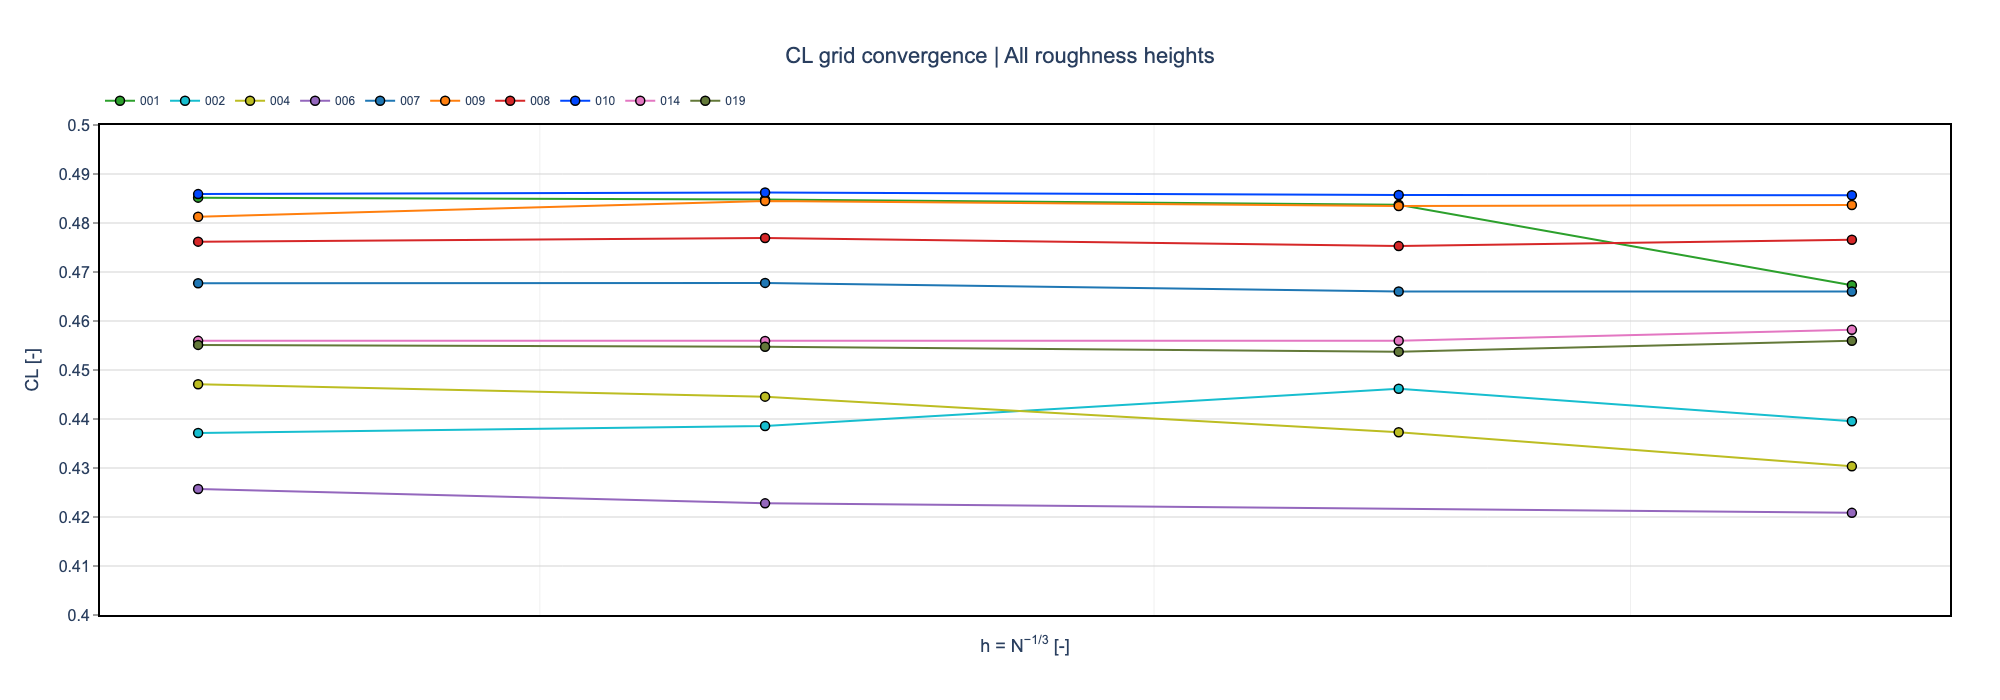
\includegraphics[width=1.0\textwidth]{FIGURES/AERODYNAMIC/tc_naca0012_ae3932_cl_vs_n_all_roughness.png}
\par}

\vspace{0.15cm}

\begin{block}{\scriptsize Assessment}
\begin{itemize}
    \item At L1, the median lift coefficient is $C_L=0.4677$, with an IQR of $0.0262$ ($5.6\%$).
    \item Most submissions exhibit limited sensitivity to spatial grid refinement.
    \item The largest coarse-grid deviations are approximately $4\%$ relative to the corresponding L1 predictions.
\end{itemize}
\end{block}

\end{frame}


% ============================================================
% NACA0012 -- Aerodynamic Grid Convergence: CD
% ============================================================

\begin{frame}{\small NACA0012 -- Drag Coefficient Grid Convergence}
\scriptsize

{\centering
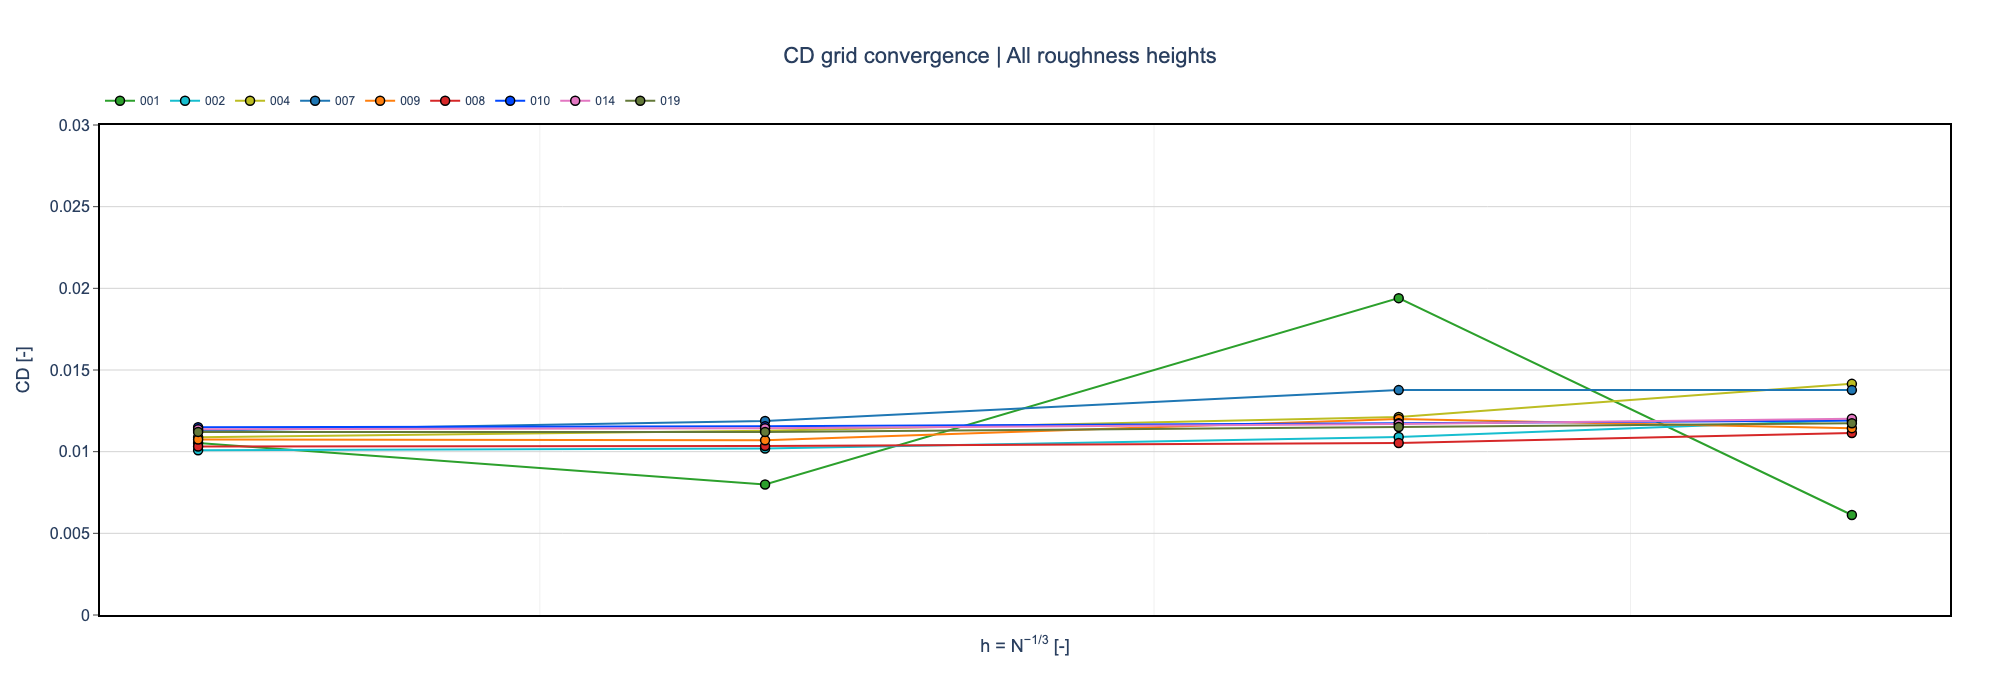
\includegraphics[width=1.0\textwidth]{FIGURES/AERODYNAMIC/tc_naca0012_ae3932_cd_vs_n_all_roughness.png}
\par}

\vspace{0.15cm}

\begin{block}{\scriptsize Assessment}
\begin{itemize}
    \item At L1, the median drag coefficient is $C_D=0.01088$, with an IQR of $7.57\times10^{-4}$ ($7.0\%$).
    \item $C_D$ exhibits greater sensitivity to spatial grid refinement than $C_L$.
    \item Non-monotonic grid-convergence behavior is observed for selected submissions.
\end{itemize}
\end{block}

\end{frame}


% ============================================================
% NACA0012 -- Aerodynamic Grid Convergence: CM
% ============================================================

\begin{frame}{\small NACA0012 -- Pitching Moment Grid Convergence}
\scriptsize

{\centering
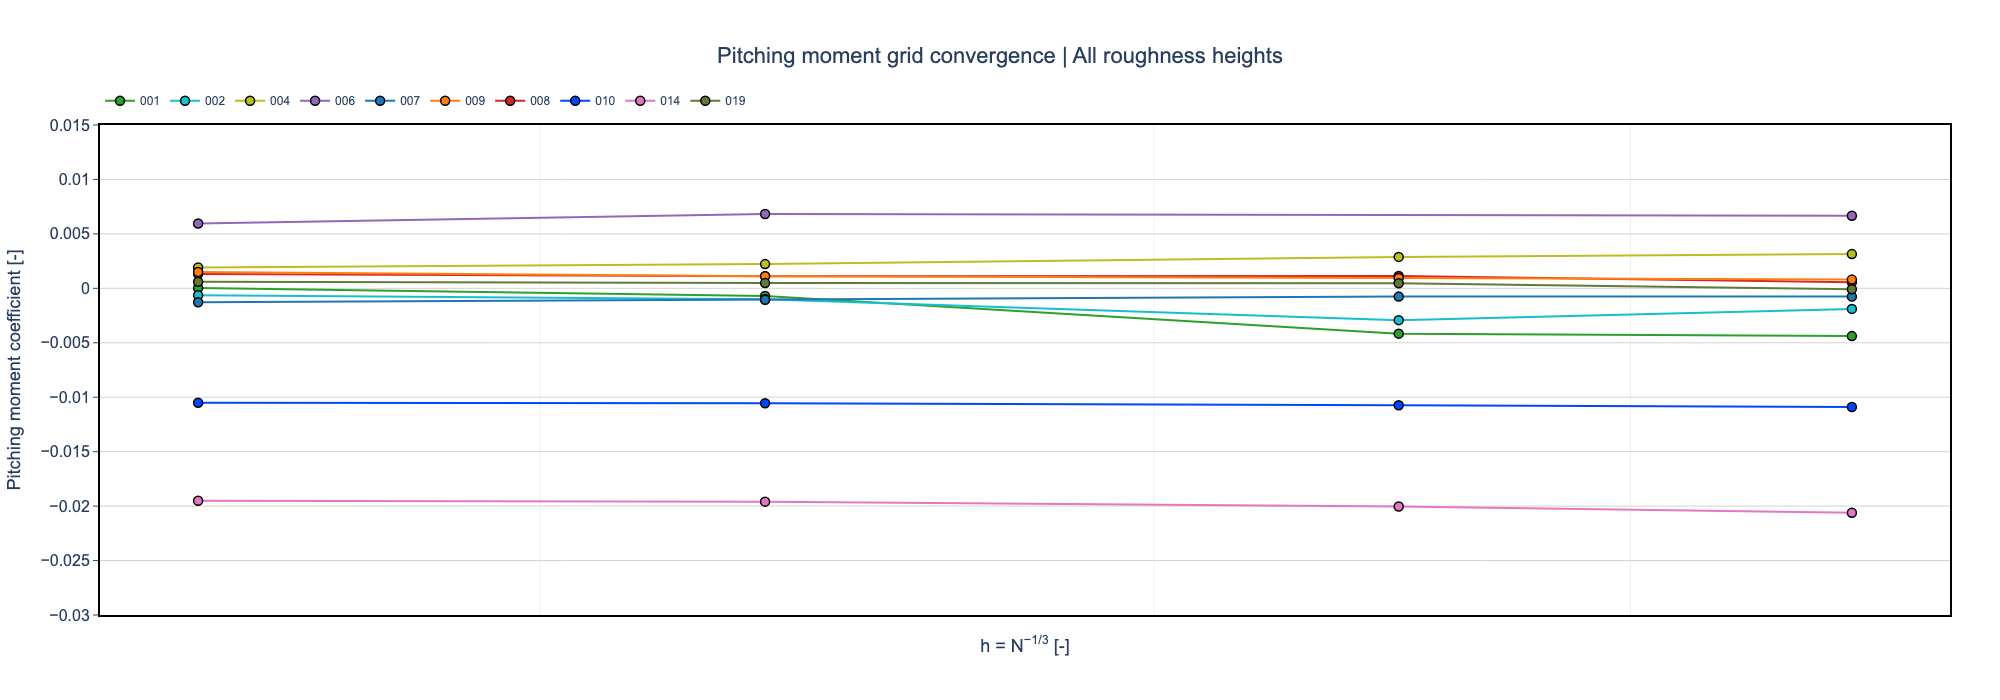
\includegraphics[width=1.0\textwidth]{FIGURES/AERODYNAMIC/tc_naca0012_ae3932_cmy_vs_n_all_roughness.png}
\par}

\vspace{0.15cm}

\begin{block}{\scriptsize Assessment}
\begin{itemize}
    \item At L1, the median pitching-moment coefficient is $C_M\approx0$, with an IQR of $2.60\times10^{-3}$.
    \item Most individual submissions exhibit limited sensitivity to spatial grid refinement.
    \item Code-to-code offsets are larger than the grid-refinement effect for most submissions.
    \item Relative percentage differences are not meaningful for $C_M$ because the reference values are close to zero.
\end{itemize}
\end{block}

\end{frame}


% ============================================================
% NACA0012 -- Surface Pressure Distribution
% ============================================================

\begin{frame}[shrink]{\small NACA0012 -- Surface Pressure Distribution (L1)}
\scriptsize

{\centering
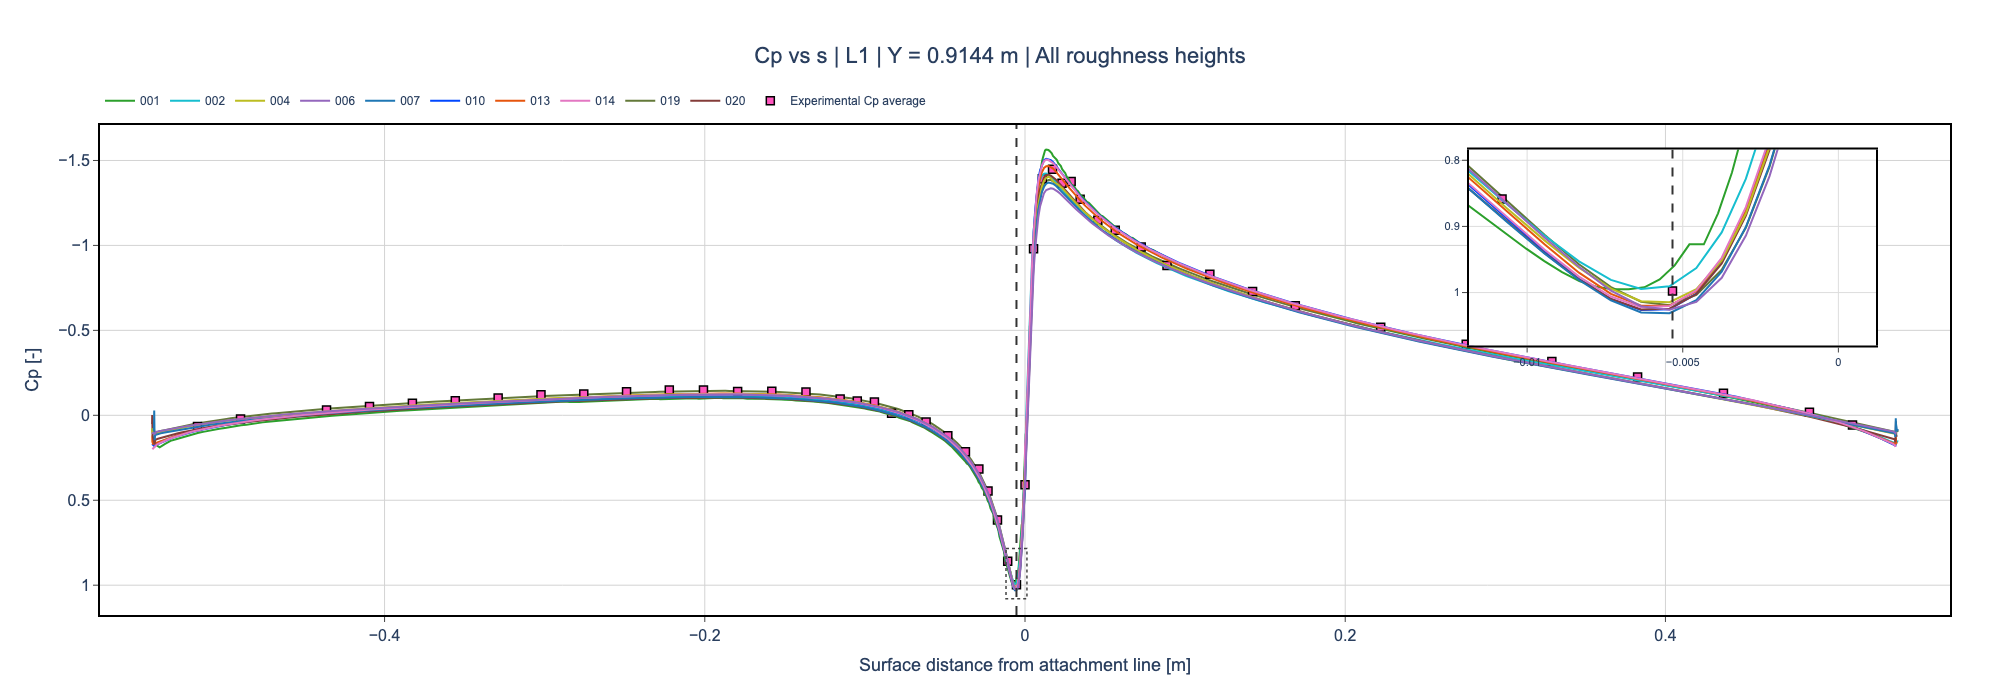
\includegraphics[width=1.0\textwidth]{FIGURES/AERODYNAMIC/tc_naca0012_ae3932_L1_cp_vs_s_slice_0p9144_all_roughness.png}
\par}

\vspace{0.15cm}

\begin{block}{\scriptsize Assessment}
\begin{itemize}
    \item The submitted $C_p$ distributions are closely clustered and show good agreement with the experimental measurements over most of the airfoil.
    \item The largest code-to-code differences are concentrated near the leading-edge suction peak and stagnation region.
    \item The overall pressure distribution is consistent across submissions despite differences in prescribed surface roughness.
\end{itemize}
\end{block}

\end{frame}


% ============================================================
% NACA0012 -- Aerodynamic Assessment Summary
% ============================================================

\begin{frame}{\small NACA0012 -- Aerodynamic Assessment Summary}
\scriptsize

\begin{block}{\scriptsize Grid Convergence}
\begin{itemize}
    \item \textbf{$C_L$:} generally weak grid sensitivity, with most submissions remaining close to their L1 prediction.
    \item \textbf{$C_D$:} greater grid sensitivity, with non-monotonic behavior observed for selected submissions.
    \item \textbf{$C_M$:} generally limited within-code grid sensitivity, while code-to-code offsets remain comparatively large.
\end{itemize}
\end{block}

\vspace{0.15cm}

\begin{block}{\scriptsize Code-to-Code Variability at L1}
\begin{center}
\begin{tabular}{lccc}
\toprule
 & \textbf{Median} & \textbf{IQR} & \textbf{Relative IQR} \\
\midrule
$C_L$ & $0.4677$    & $0.0262$                & $5.6\%$ \\
$C_D$ & $0.01088$   & $7.57\times10^{-4}$     & $7.0\%$ \\
$C_M$ & $\approx 0$ & $2.60\times10^{-3}$     & -- \\
\bottomrule
\end{tabular}
\end{center}

\vspace{0.05cm}

\centering
\textit{Relative IQR is not reported for $C_M$ because normalization by a value close to zero is ill-conditioned.}
\end{block}

\vspace{0.15cm}

\begin{alertblock}{\scriptsize Aerodynamic Takeaway}
The $C_p$ distributions are closely clustered and generally agree well with the experimental measurements. Grid refinement produces relatively small changes in $C_L$ and $C_M$ for most submissions, while $C_D$ is more grid-sensitive. Residual code-to-code differences therefore cannot be attributed to spatial resolution alone.
\end{alertblock}

\end{frame}


% ============================================================
% ============================================================
% END -- NACA0012 AERODYNAMIC GRID CONVERGENCE
% ============================================================
% ============================================================
